\definecolor{MidnightBlue}{cmyk}{0.98,0.13,0,0.43} % PANTONE 302

% MidnightBlue with white lettering is cool!
\pagecolor{MidnightBlue}
\color{white}

\begin{center}
{\Huge From Algorithms to Z-Scores: 

\bigskip

Probabilistic and Statistical Modeling in Computer Science}

\bigskip

{\LARGE Norm Matloff, University of California, Davis}

\medskip

\end{center}

\vspace{0.4in}

\begin{center}
\begin{figure}[ht]
\color{white}
   \begin{minipage}[b]{0.55\linewidth}
       \Large
       $
       \mbox{\boldmath$ f_X(t) = c e^{-0.5 (t-\mu)'\Sigma^{-1}(t-\mu)}$ } 
       $
   \end{minipage}
   \hspace{0.1in}
   \begin{minipage}[b]{0.58\linewidth}
       {\bf
       \begin{Verbatim}[fontsize=\relsize{+1}]
       library(MASS) 
       x <- mvrnorm(mu,sgm)
       \end{Verbatim}
       }
   \end{minipage}
\end{figure}
\end{center}

\vspace{-1.75in}
\begin{center}
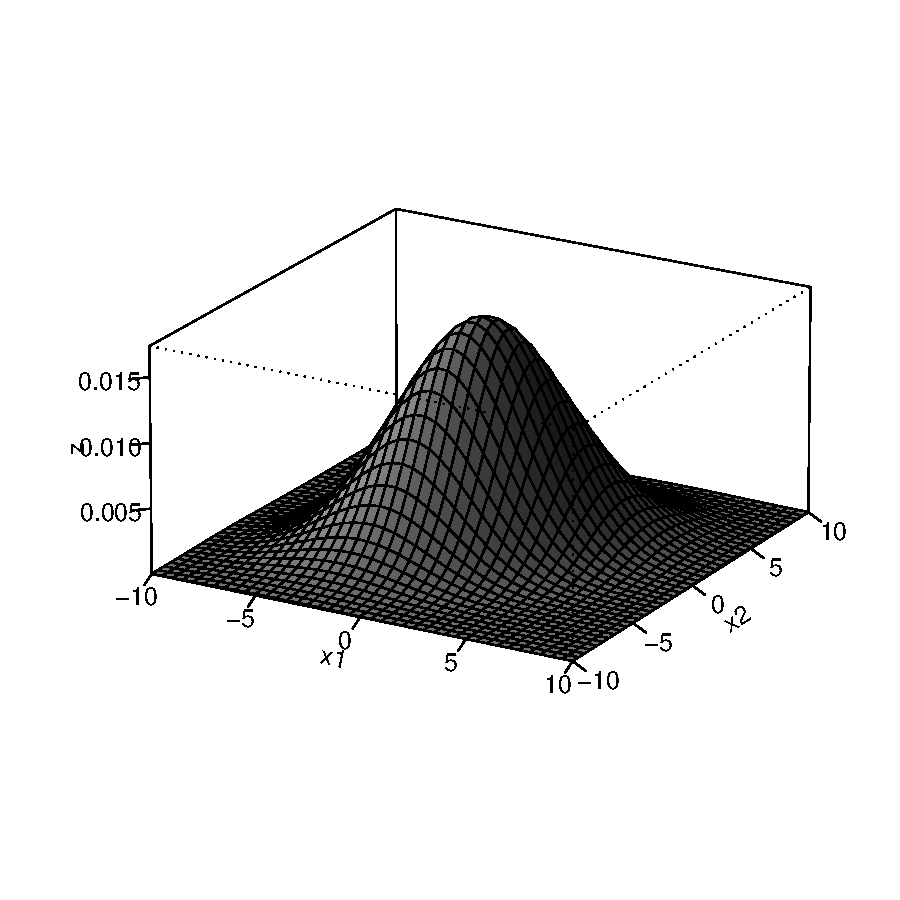
\includegraphics[width=4.8in]{Bell.pdf}

{See Creative Commons license at \\ 
\vspace{0.2in}
{http://heather.cs.ucdavis.edu/~matloff/probstatbook.html}
}

The author has striven to minimize errors, but no guarantee is made as to
accuracy.  

\end{center}

{\bf THIS IS THE BRIEF EDITION; FULL TEXT AT ABOVE URL.  
A FEW REFERENCES TO FULL TEXT APPEAR AS QUESTION MARKS.}

